\documentclass[12pt,titlepage]{article}
\usepackage[ngerman]{babel}
\usepackage[utf8]{inputenc}
\usepackage{color}
\usepackage[a4paper,lmargin={2cm},rmargin={2cm},tmargin={2.5cm},bmargin = {2.5cm}]{geometry}
\usepackage{amssymb}
\usepackage{amsthm}
\usepackage{graphicx}
\usepackage[section]{placeins}
\title{
\includegraphics[width=0.3\textwidth]{images/bibnow-logo-monotone.png}}
\author{Jawoon Kim, Charlie Wiegand}
\begin{document}
    \begin{titlepage}
    \centering
    
\includegraphics[width=0.3\textwidth]{images/bibnow-logo-monotone.png}\par\vspace{1cm}
    {\scshape\LARGE bib International College\par}
    \vspace{1cm}
    {\rmfamily\scshape Lernaufgabe 2020\par}
    \vspace{1.5cm}
    {\Huge\bfseries bib now\par}
    \vspace{2cm}
    {\Large\itshape Charlie Wiegand\par Jawoon Kim\par}
    \vfill
    betreut von Frau Langeheinecke\par
    \vfill
    {\large \today\par}
    \end{titlepage}

\tableofcontents
\newpage

\addcontentsline{toc}{section}{Abbildungsverzeichnis}
\listoffigures

\pagebreak


\maketitle

\vspace{2cm}


\section{Über bibnow}


bib-now, das Forum, das exclusive Forum für alle Studierenden und Mitarbeiter.

\vspace{1cm}

Erstellt von Jawoon Kim und Charlie Wiegand(PBT3H19A).

Letzte Revision: September 2020

\vspace{2cm}

\begin{quote}
\textbf{Note}

Diese Version enthält die Dokumentation der Webseite und Erläuterungen. Sie dient
der Einarbeitung in bib-now sowie dem Verständnis der Konzepte. 
\end{quote}

\pagebreak

\section{Aufgabenstellung}


Da zur Zeit häufig Mails an die ganze Schule geschickt werden, wenn beispielsweise jemand etwas verloren hat, wollen wir unseren Mitschülern und uns ein Forum bieten, das diesen Austausch erleichtert.

Für dieses Vorhaben haben wir uns folgende Ziele und Richtlinien gesetzt

\begin{itemize}
\item
\textbf{Minimum}
  Es soll eine lauffähige Webseite erstellt werden, auf der man sich mindestens einloggen kann und anschließend Beiträge in Textform hochladen kann. 
\item
\textbf{Optional}
  Es soll die Möglichkeit geben seine Beiträge durch Bilder zu ergänzen und die Posts sollen in Kategorien eingeteilt werden
\item
\textbf{Optional}
Desweiteren soll es die Möglichkeit den Stundenplan und Klausurplänung aus dem offiziellen Intranet zu übernehmen.

\end{itemize}


\textbf{Vorausetzungen}
Um das Minimum zu erreichen benötigen wir einen PC, einen Texteditor, npm, ein AngularFramework und Firebase. Um uns die Zusammenarbeit zu erleichtern haben wir uns entschieden Versionskontrolle über git laufen zu lassen und die Ergebnisse über GitHub auszutauschen. 

\newpage
\section{Konzepte}

\subsection{Inhaltskonzept}

\vspace{2cm}

\begin{figure}[hbt!]
 \centering
 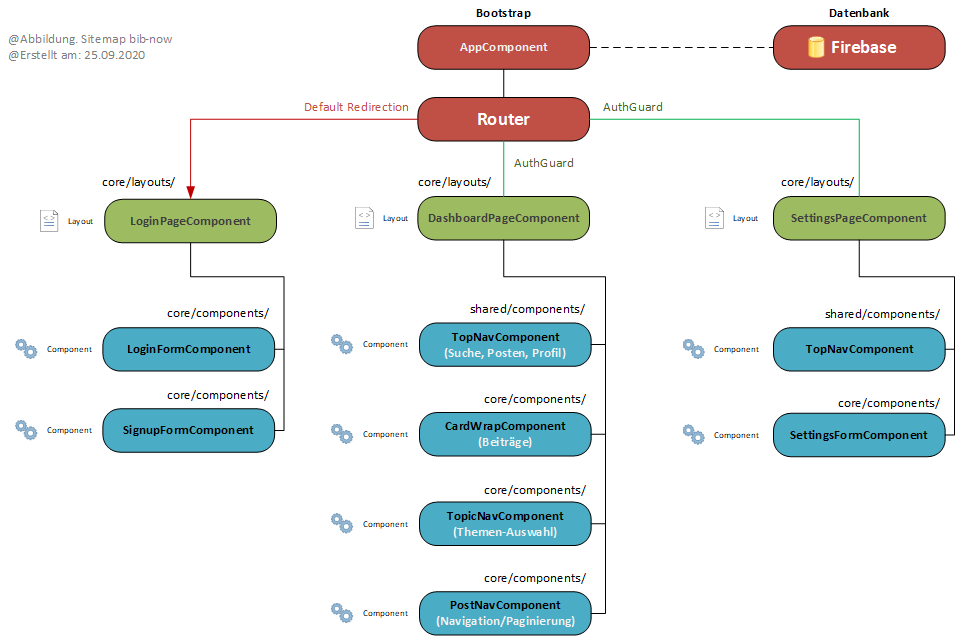
\includegraphics[width=400pt]{abbildungen/Abbildung_Sitemap.png}
 \caption{Sitemap}
\end{figure}


\vspace{2cm}

Bei bib-now handelt es sich um ein Schülerforum für das bib international College Paderborn. Die technische Umsetzung basiert auf  einer Single-Page-Webanwendung mit einer RealTime-Datenbank deren einzelnde Komponenten über einen Router verlinkt sind: Die Navigation besteht aus drei Komponenten: LoginPageComponent, DashboardPageComponent und der SettingsPageComponent. Jede dieser Komponenten besitzt ihre eigenen Backend-Komponenten. Die LoginPage greift auf die LoginFormComponent und SignUpFormComponent zurück. Die DashboardPageComponent greift auf  SideNavComponent, ForumComponent, PostComponent zurück. Außerdem könnnen hier später weitere Elemente ergänzt werden. SettingsPageComponent beinhaltet die SideNavComponent und SettingsFormComponent. 


\FloatBarrier

\subsection{Navigationskonzept}

\vspace{2cm}

\begin{figure}[hbt!]
\centering
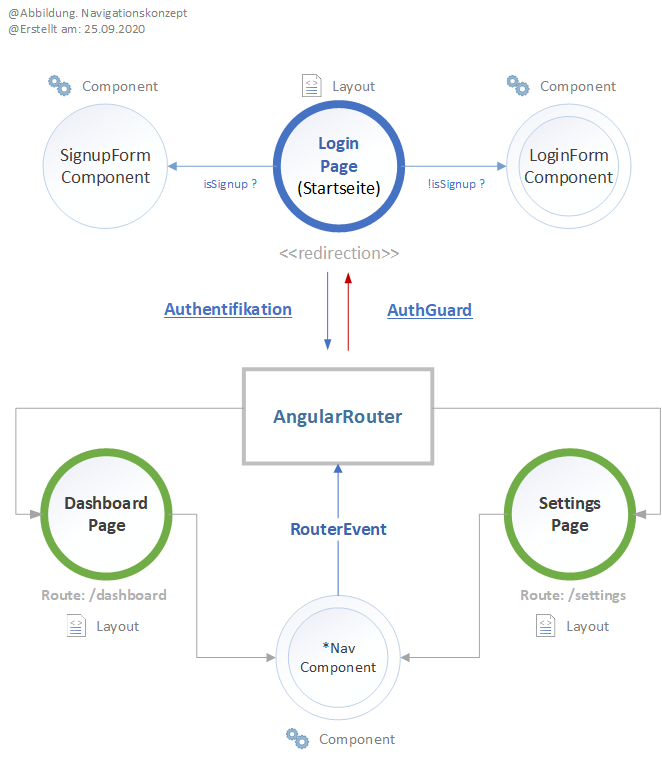
\includegraphics [width=400pt]{abbildungen/Abbildung_Navigationskonzept.png}
\caption{Navigationskonzept}
\end{figure}


\vspace{2cm}


Beim Betreten der Seite wird der User zunächst aufgefordert sich einzuloggen. Sollte er sich noch nicht registriert haben hat er die Möglichkeit in das Registrierungsforumlar zu switchen und sich dort zu registrieren. War die Registrierung oder das einloggen erfolgreich, wird der User auf die DashboardPage weitergeleitet. Dort werden ihm Posts angezeigt und er hat die Möglichkeit über ein Formular einen eigenen Post zu verfassen. Außerdem kann er über das Navigationsmenu zu der SettingsPage zu wechseln. Seine aktuelle Position wird durch eine Farbveränderung am jeweiligen punkt in der Navigatonsleiste erkenntlich.

\FloatBarrier
\subsection{Gestaltungskonzept}

Font: Montserrat (https://fonts.google.com/specimen/Montserrat)
Font Weights: 100, 300, 700
\vspace{2cm}
\begin{itemize}
\item
	Für Subtitel, gedämpfte Texte, etc

\begin{figure}[hbt!]

\includegraphics{images/Schriftart_100.png}
\caption{Schriftart 100}
\end{figure}
\item
	Für normale Texte, Standard-schriftart

\begin{figure}[hbt!]

\includegraphics{images/Schriftart_300.png}
\caption{Schriftart 300}
\end{figure}
\item
	Für Titel und Akzent(Betonung)

\begin{figure}[hbt!]

\includegraphics{images/Schriftart_700.png}
\caption{Schriftart 700}
\end{figure}
\end{itemize}


Farbenschema

Schemakonzept: Neon + Material

Primärfarbe:\#D43D61

Sekundär:\#039BE5

Hintergrund:\#271D33

Hintergrund Beiträge:\#F8F6F6

\begin{figure}[hbt!]
\centering
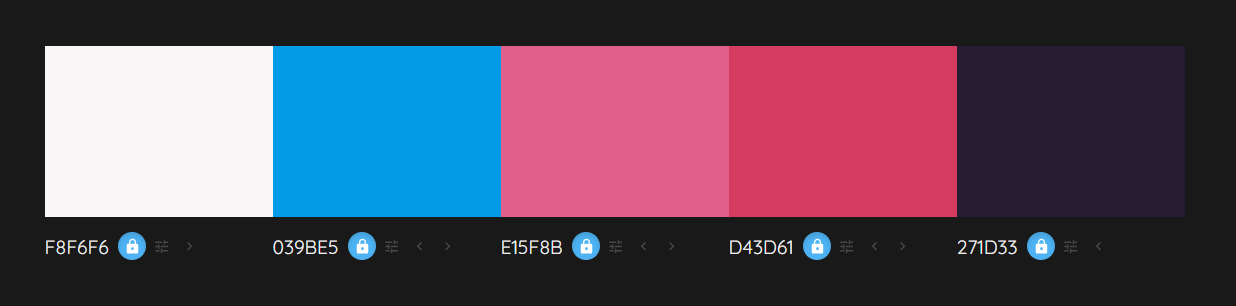
\includegraphics[width=400pt]{images/Schema_1.png}
\caption{Farbenschema}
\end{figure}

\FloatBarrier

\subsection{Zielgruppendefinition}

Aus den MUSS - und KANN-Zielen ergibt sich unsere Zielgruppe: alle Schüler und Mitarbeiter des bib international College Paderborn. 

\newpage
\section{Durchführung}

\subsection{Allgemeine Beschreibung zur Durchführung}

Beim Entwickeln der Webseite  haben wir uns täglich Abgesprochen welche Features wir als nächstes brauchen und diese in Form von  Backend und Frontend unter uns aufgeteilt. Da wir über GitHub gearbeitet haben konnten wir beide unsere branches pushen und mit dem Master-Branch auf konfliktfreie Kompatibiltät prüfen und anschließend testen.

\subsection{Planung und Vorbereitung}

\subsubsection{Vor dem Projekt}

Corona bedingt wurden wir erst recht spät über die LEA informiert. Wir haben die Zeit die wir dennoch noch zur Vorbereitung hatten, genutzt um uns über Nutzung des Frameworks Angular sowie die dortige implementierung von Firebase Funktionen zu informieren. Dies geschah in Form von diversen Youtube-Videos sowie dem Durchstöbern der jeweiligen Dokumentationen.\\ \\
Wir sind davon ausgegangen, dass wir eine lauffähige Webseite mit den minimal Anforderungen in den ersten Tagen realisieren können und uns anschließend mit den optionalen Zielen und der Dokumentation beschäftigen können.

\subsubsection{Während des Projekts}

Zu Beginn haben wir die Dateistruktur sowie den Ablauf abgesprochen. Wir haben uns darauf geeinigt, dass wir die Anwendung der Seite zurnächst in Core und Shared unterteilen. Der Core-Ordner soll außerdem in Components und Layouts unterteilt werden, um eine physische Trennung von Logik und Frontend zu erzielen. Der Shared-Ordner soll alle restlichen Komponenten enthalten unterteilt in ihre jeweilen Oberkategorien: Models, Guards, Services, Module und Components die in das Core Modell integriert werden. \\ \\

Außerdem haben wir am Anfang der LEA einen Plan erstellt, wann welches Modul erledigt sein soll. Da das jedoch ein sehr steifes Modell war und überhaupt nicht zu den flexiblen Problemen in der LEA gepasst hat, haben wir das Modell schussendlich nur als grobe Richtlinie gesehen und unsere Planung für den Tag an die gerade benötigten Aufgaben angepasst.

\newpage
\section{Ergebnis}

\subsection{GitHub-Pfad}

Der Source-Code zum Ergebnis lässt sich unter folgendem Pfad finden: \\
https://github.com/bib-lea/bib-now

\subsection{Loginseite}

Auf der Loginseite hat der Nutzer drei mögliche Ansichten zwischen denen er hin und her wechseln kann. Eine Auswahl zwischen Anmeldung und Registrierung in Form von Buttons, ein Registrierfoumlar und ein Anmeldeformular.

Beim Abschicken des Registrierungsforumalar wird ein Nutzer in der Datenbank erzeugt. Beim Abschicken des Anmeldeformulars wird geprüft ob der Nutzer mit diesen Daten in der Datenbank hinterlegt ist. Ist das der Fall ändert sich der Authentifzierungsstatus und der Nutzer wird zur Dashboardseite weitergeleitet. Ist das nicht der Fall bleibt der Nutzer auf der Loginseite.

\begin{figure}[hbt!]
\centering
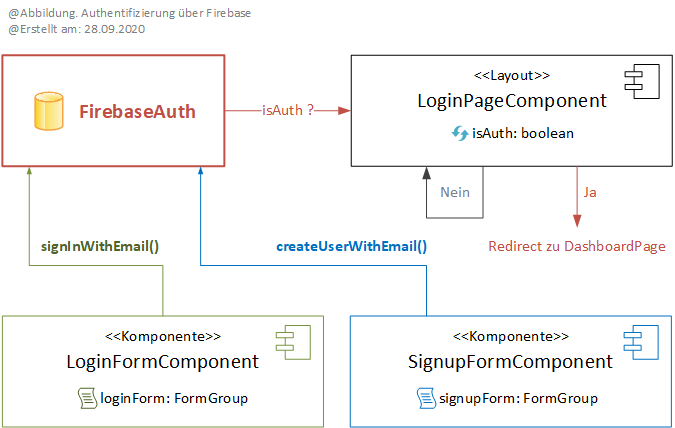
\includegraphics[width=400pt]{abbildungen/Abbildung_Authentifizierung_LoginPage.png}
\caption{Authentifizierung über FIrebase}
\end{figure}

\FloatBarrier
\newpage
\subsubsection{Desktop Ansicht}

\begin{figure}[hbt!]
\centering
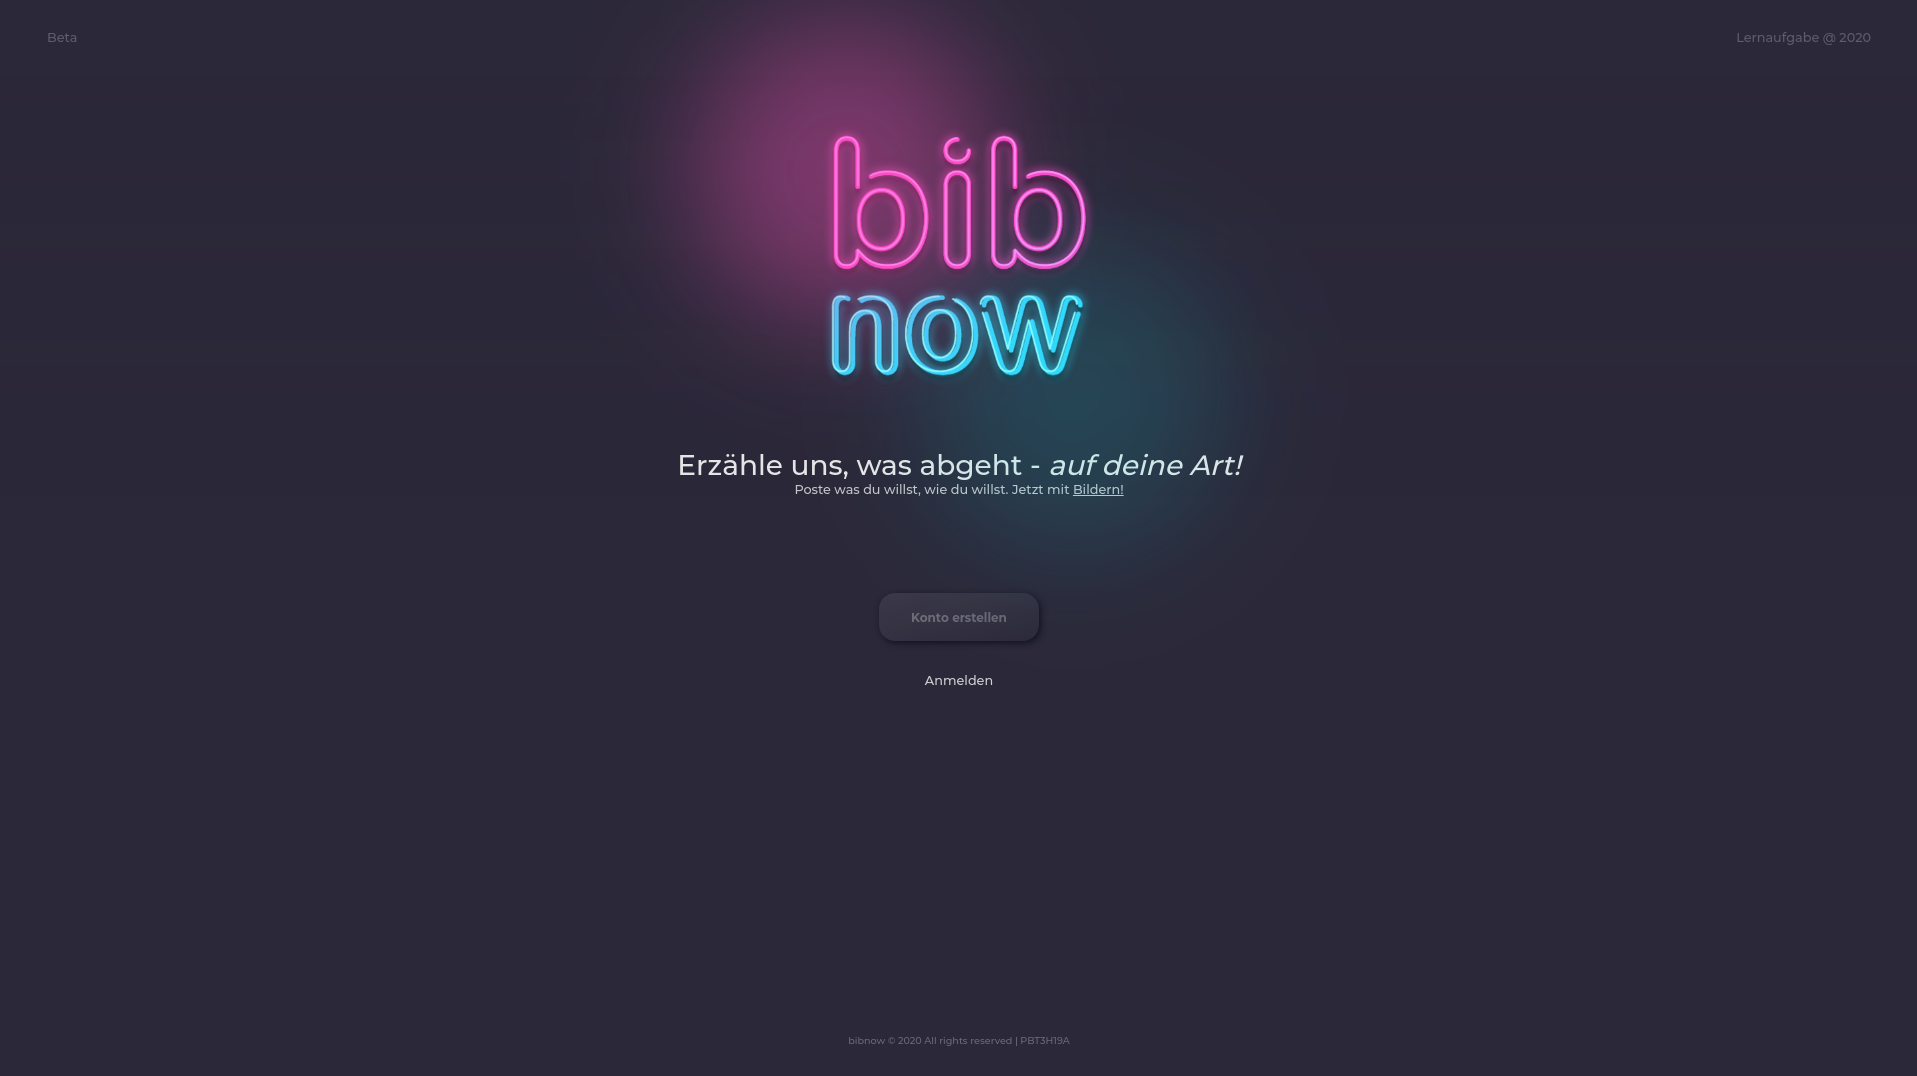
\includegraphics[width=400pt]{screenshots/Screenshot_Desktop1.png}
\caption{Screenshot LandingPage Desktop}
\end{figure}

\begin{figure}[hbt!]
\centering
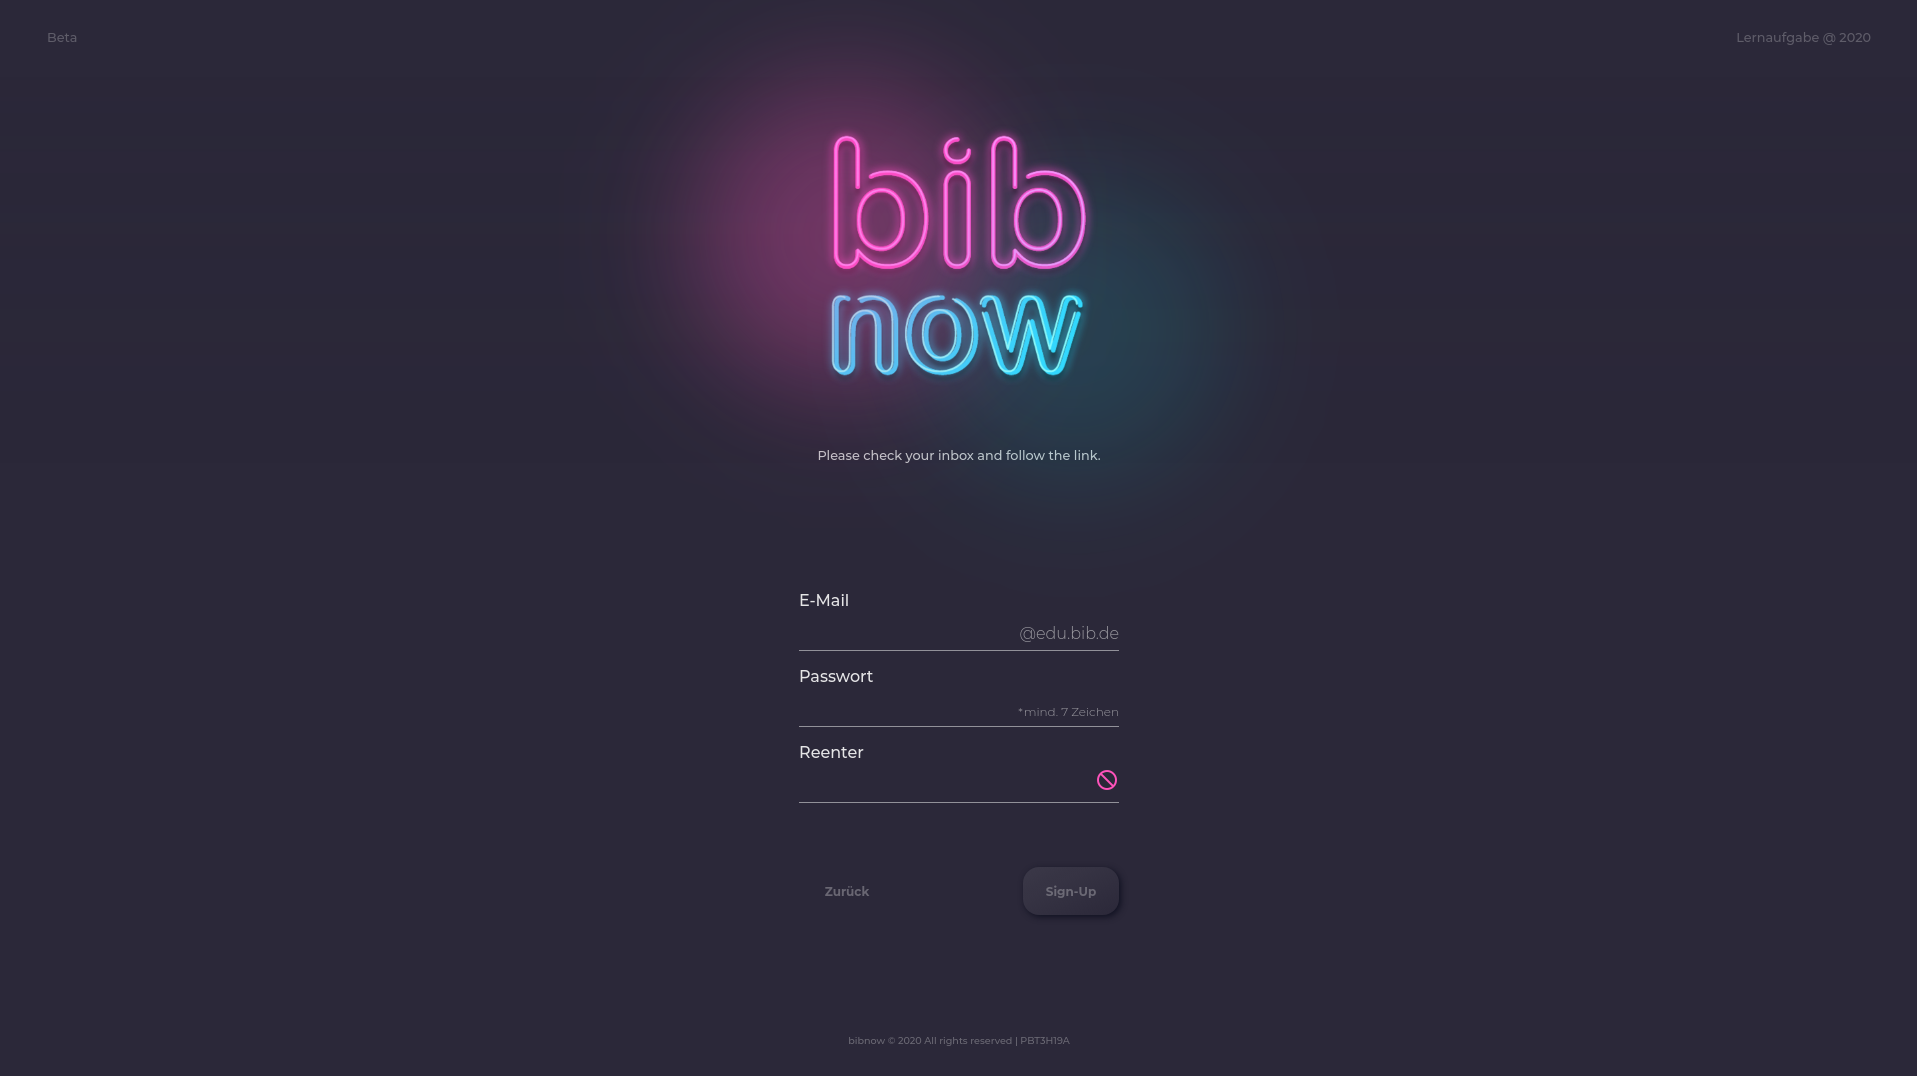
\includegraphics[width=400pt]{screenshots/Screenshot_Desktop2.png}
\caption{Sreenshot Registrierung Desktop}
\end{figure}

\begin{figure}[hbt!]
\centering
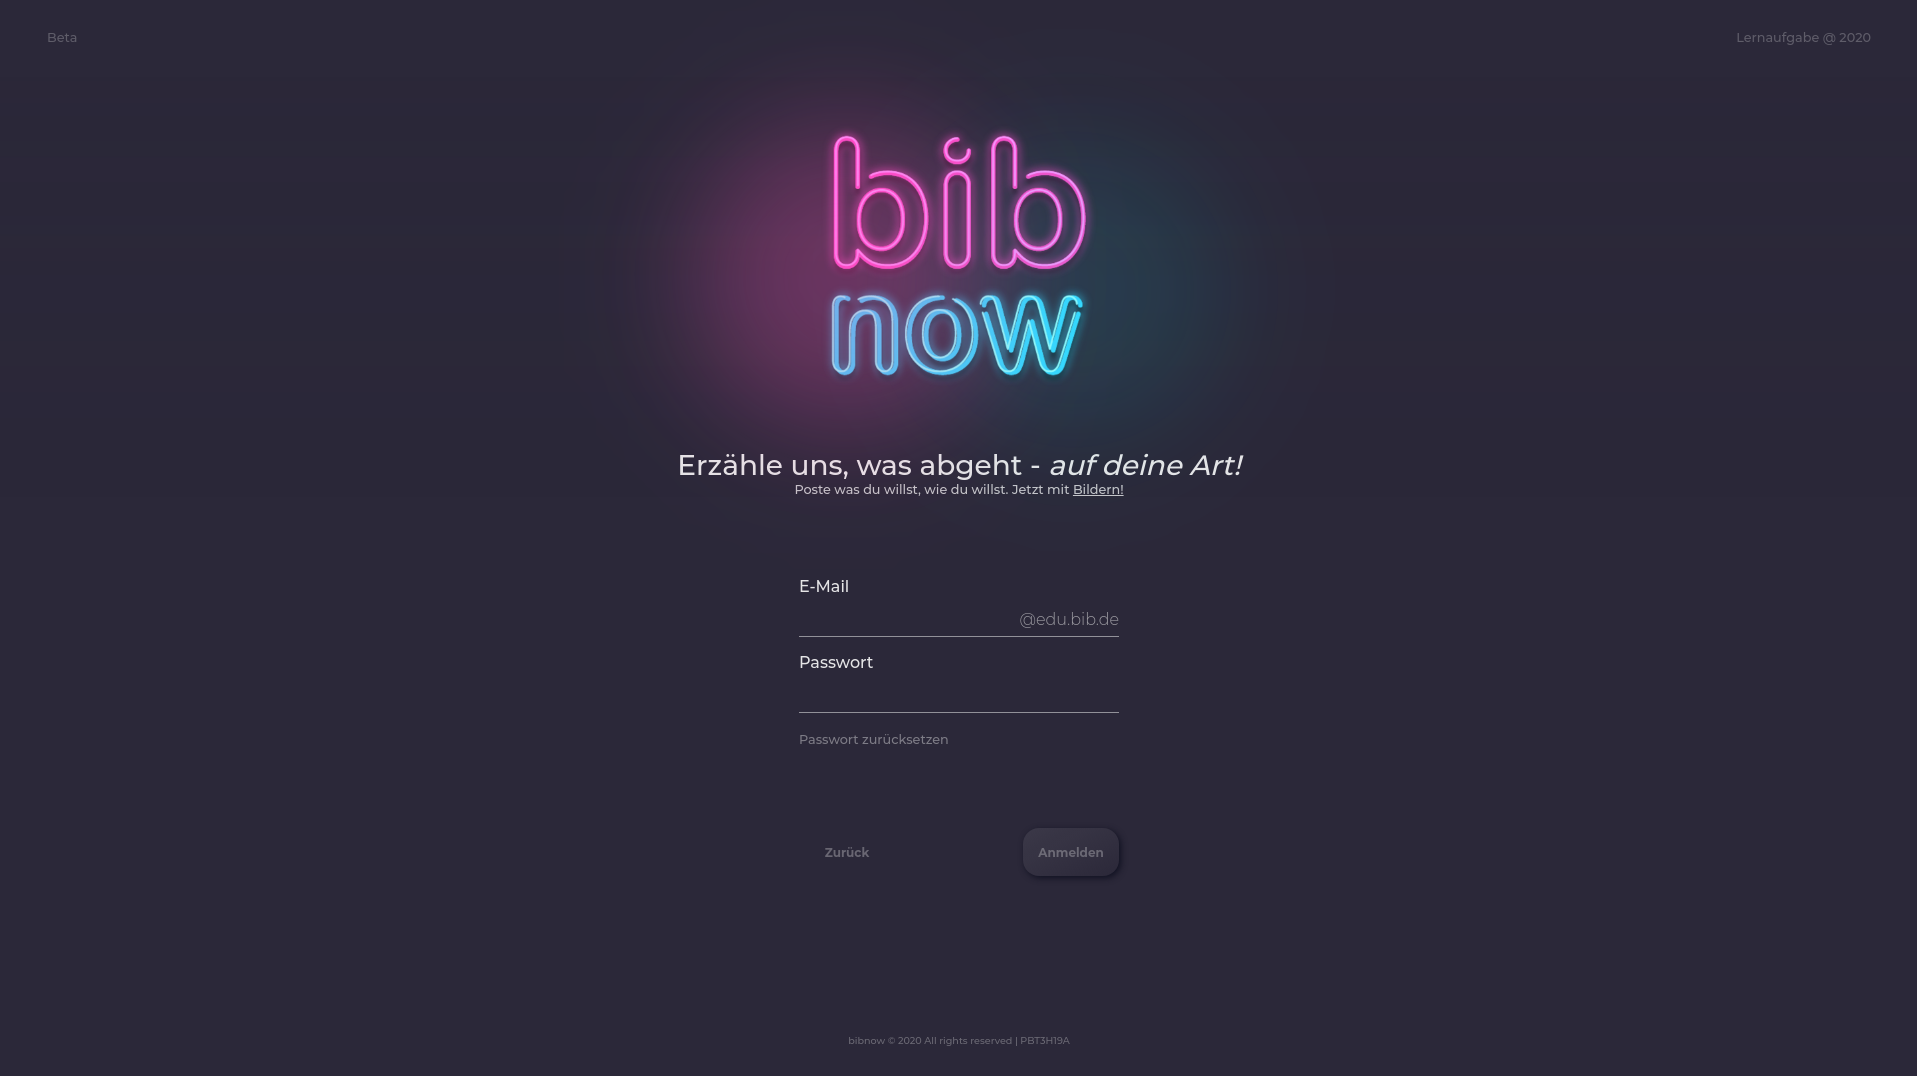
\includegraphics[width=400pt]{screenshots/Screenshot_Desktop3.png}
\caption{Screenshot Anmeldung Desktop}
\end{figure}

\FloatBarrier

\newpage

\subsubsection{Mobile Ansicht}

\begin{figure}[hbt!]
\centering

\includegraphics[width=150pt]{screenshots/Screenshot_Mobil1.png}
\caption{Screenshot LandingPage Mobil}
\end{figure}

\begin{figure}[hbt!]
\centering
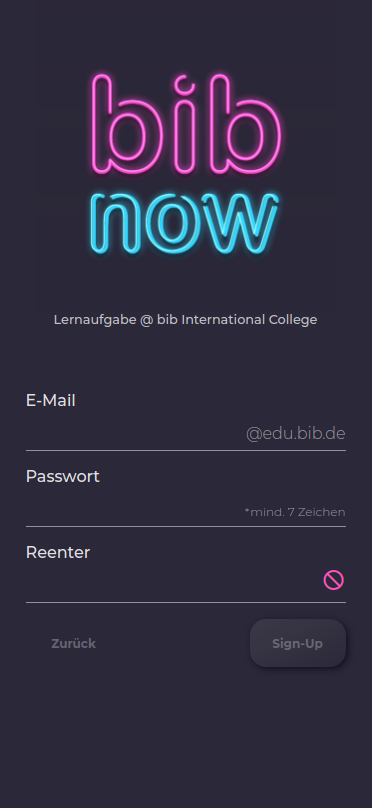
\includegraphics[width=150pt]{screenshots/Screenshot_Mobil2.png}
\caption{Sreenshot Registrierung Mobil}
\end{figure}

\begin{figure}[hbt!]
\centering

\includegraphics[width=150pt]{screenshots/Screenshot_Mobil3.png}
\caption{Screenshot Anmeldung Mobil}
\end{figure}

\FloatBarrier

\subsection{Dashboard}

Auf dem Dashboard ist eine Navigationsleiste, die ContentViewer Komponente und der Footer zu sehen. In der Navigationsleiste ist das Logo, eine Suchfunktion, die nach Schlüsselworten in den Titeln und Inhalten der Beiträge sucht, der Button um den Postdialog zu öffnen, ein Auslogg-Button, der den Nutzer wieder zur Einloggseite führt. Die ContentViewer Komponente zeigt oben eine Auswahl zwischen Fundbüro und Tutorium, um Posts der jeweiligen Kategorie anzuzeigen und unten eine Pagination um sich weitere Posts anzusehen. Die CardWrap Komponente im ContentViewer zeigt immer fünf Posts, wobei der aktive immer durch weiße Hervorhebung markiert ist. Zu dem hat der Nutzer die Möglichkeit den Post zu löschen, sofern er der Autor ist. Dies ist durch ein Mülleimer-Icon markiert.

\begin{figure}[hbt!]
\centering
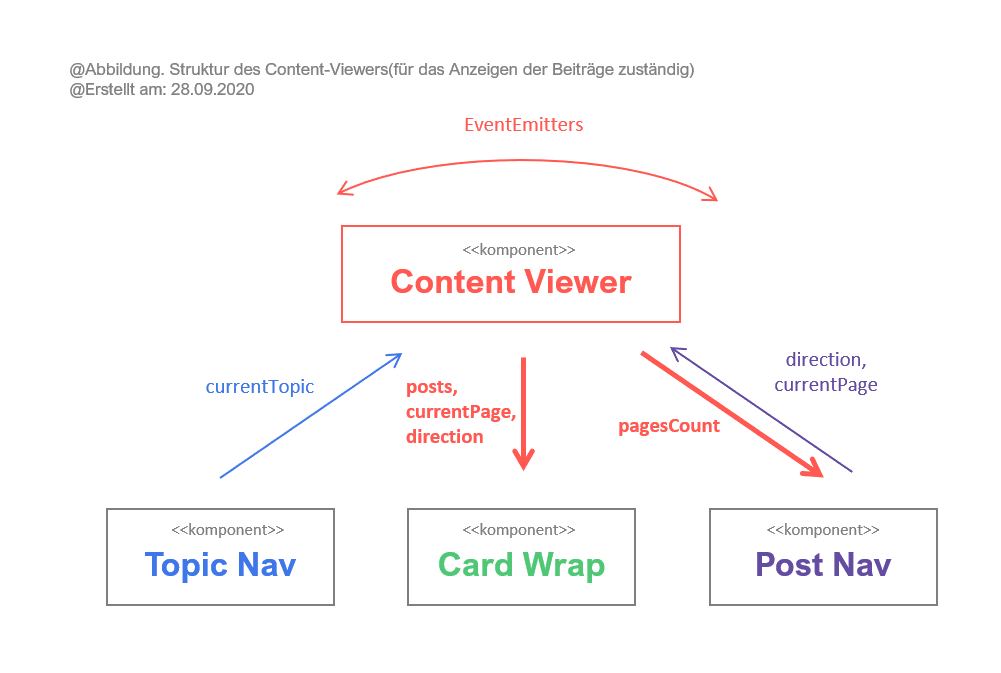
\includegraphics[]{abbildungen/Abbildung_ContentViewer.png}
\caption[ContentViewer]{ContentViewer \\Quelle: eigene Darstellung}
\end{figure}

Betätigt der Nutzer den Posten-Button öffnet sich ein Formular in dem der Nutzer sich für ein Oberthema sowie Untertypen entscheiden kann. Zudem müssen Titel und Inhalt ausgefüllt sein, damit die Daten in die Datenbank geladen werden. Ist das nicht der Fall, wird der Nutzer dazu aufgefordert dies zu tun. Die Zugabe eines Bildes ist optional. Gibt der Nutzer kein Bild an, wird ein Demobild verwendet.

\FloatBarrier
\newpage

\subsubsection{Desktop Ansicht}

\begin{figure}[hbt!]
\centering
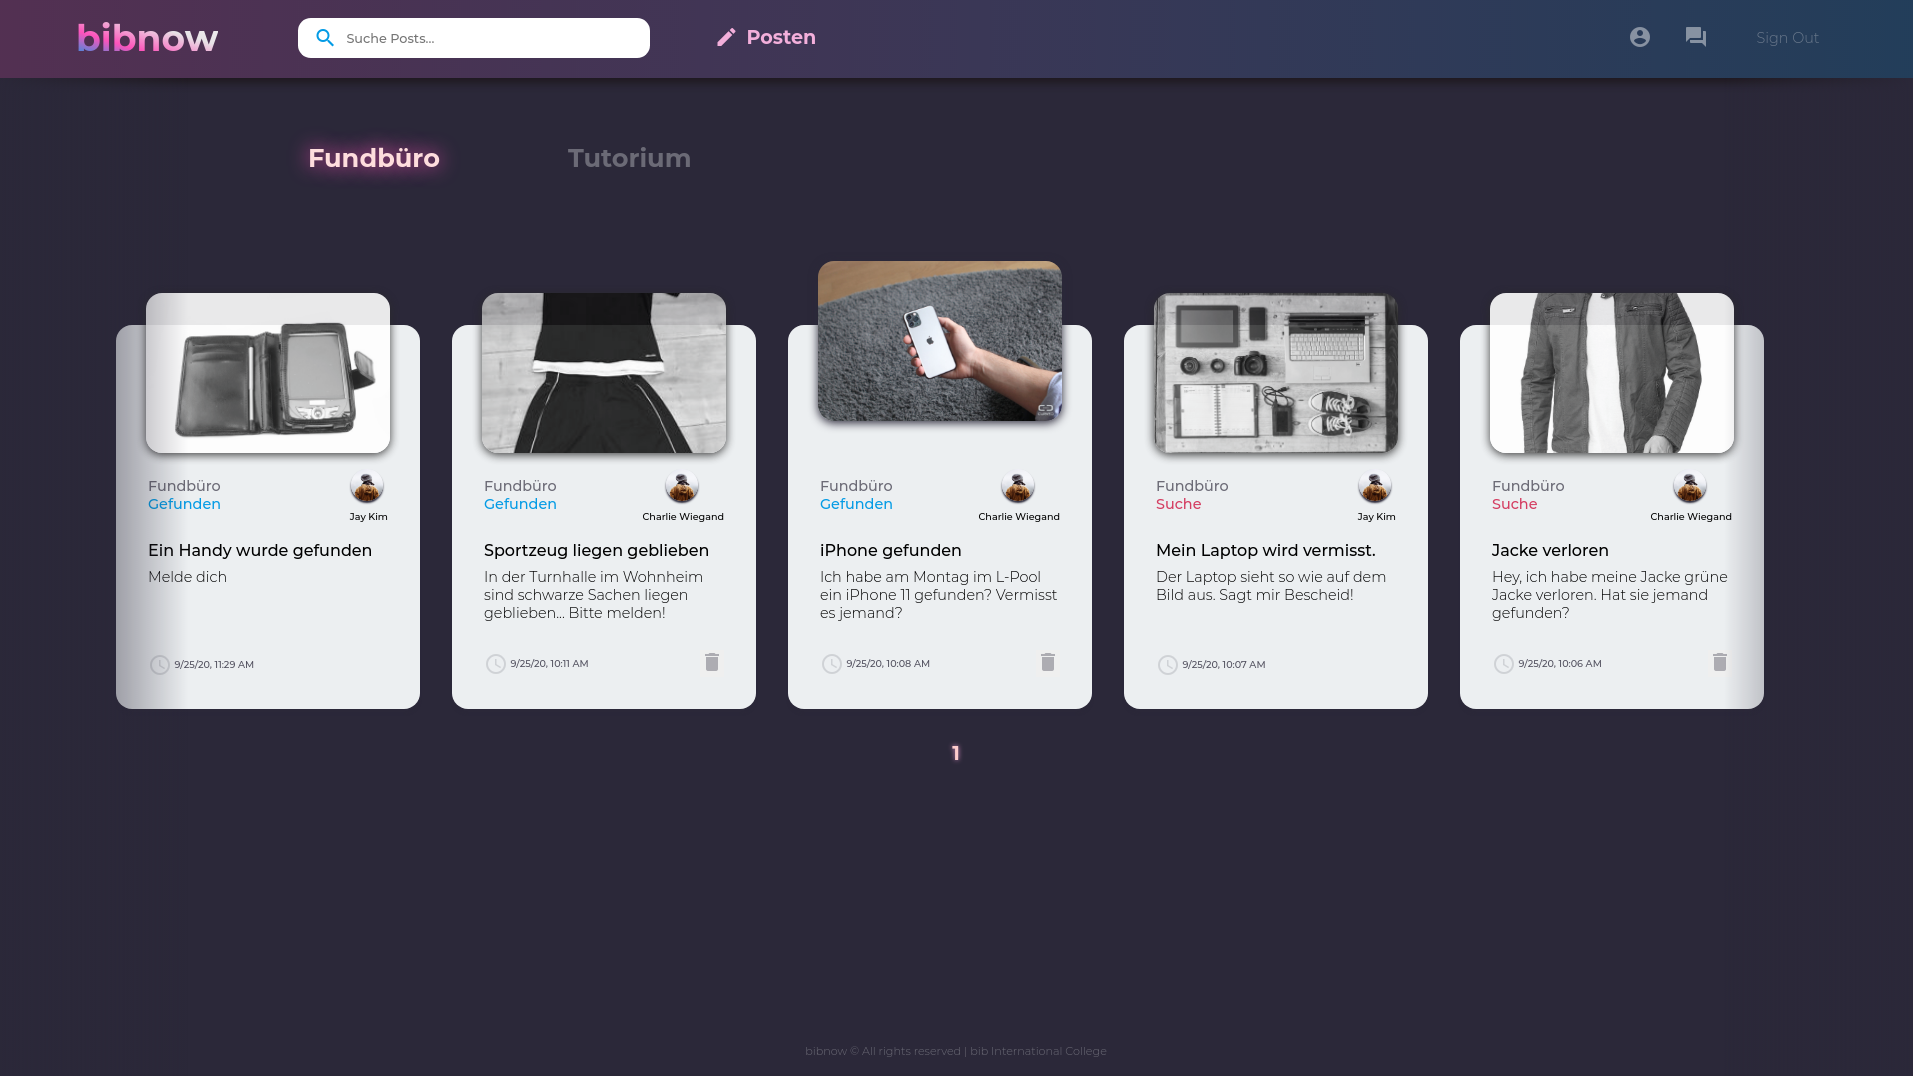
\includegraphics[width=400pt]{screenshots/Screenshot_Desktop_Dashboard.png}
\caption[Sreenshot Dashboard]{Screenshot Dashboard \\Quelle: eigene Darstellung}
\end{figure}

\begin{figure}[hbt!]
\centering
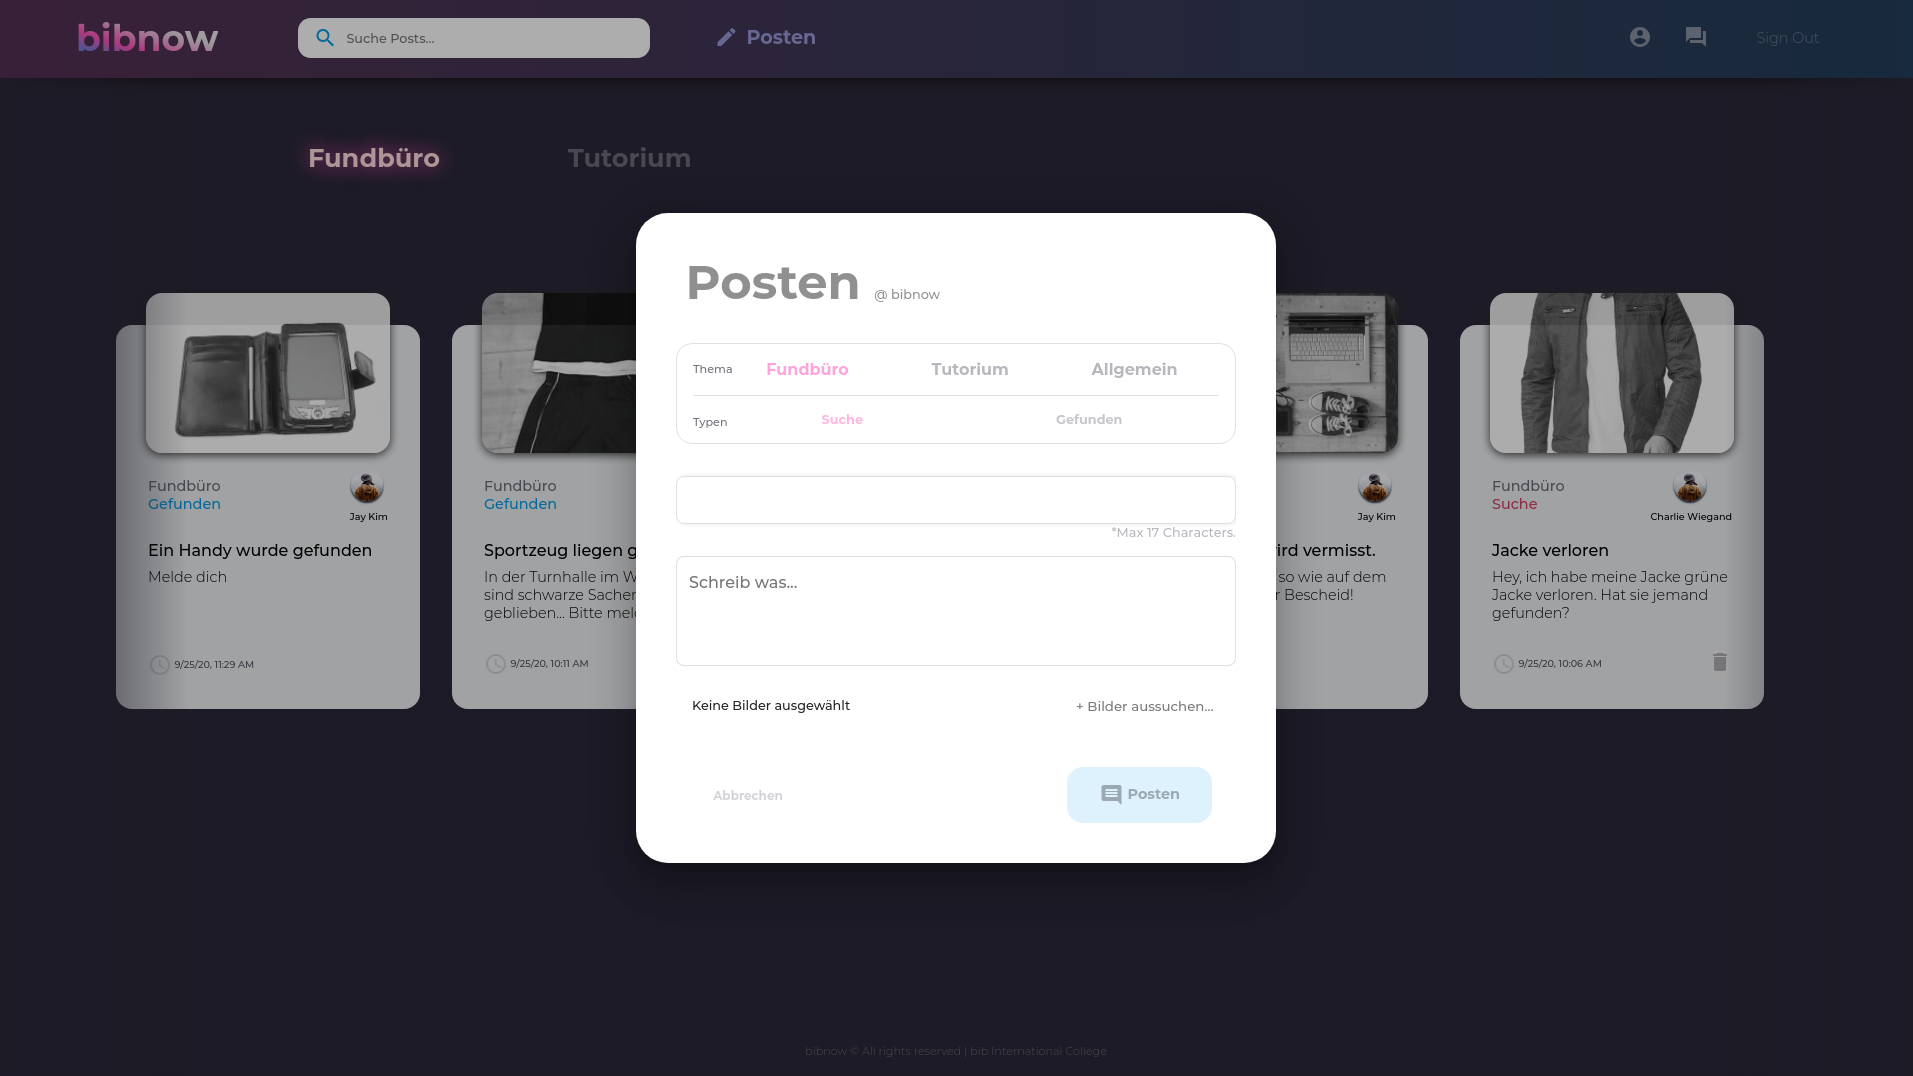
\includegraphics[width=400pt]{screenshots/Screenshot_Desktop_Posten.png}
\caption[Sreenshot Postdialog]{Screenshot Postdialog\\Quelle: eigene Darstellung}
\end{figure}

\FloatBarrier
\newpage
\subsubsection{Mobile Ansicht}

\begin{figure}[hbt!]
\centering
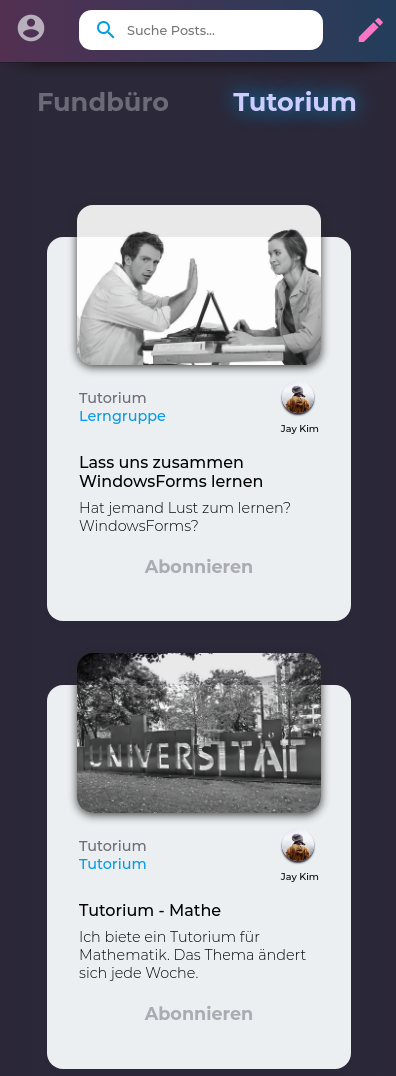
\includegraphics[width=150pt]{screenshots/Screenshot_Mobil_Dashboard.png}
\caption[Sreenshot Dashboard]{Screenshot Dashboard \\Quelle: eigene Darstellung}
\end{figure}

\begin{figure}[hbt!]
\centering
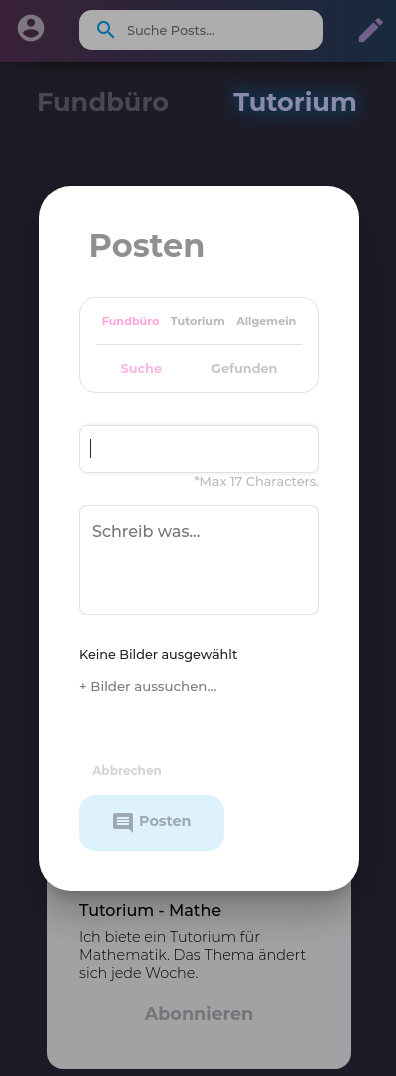
\includegraphics[width=150pt]{screenshots/Screenshot_Mobil_Posten.png}
\caption[Sreenshot Postdialog]{Screenshot Postdialog\\Quelle: eigene Darstellung}
\end{figure}

\FloatBarrier

\subsection{Datenbank}

Die Datenbank implementierung fand in Firebase statt. Dort haben wir zwei Sammlungen erstellt: eine für Posts und eine für die Userdaten. 
Nachdem sich die Bildspeicherung in einer solchen RealTime Cloud Sammlung als problematisch herausstellte, haben wir sie in einen separaten StorageBucket in Firebase geladen und anschließend den Link zu dem jeweiligen Bild als string unter dem jeweiligen Post gespeichert. 

\begin{figure}[!htb]
\centering
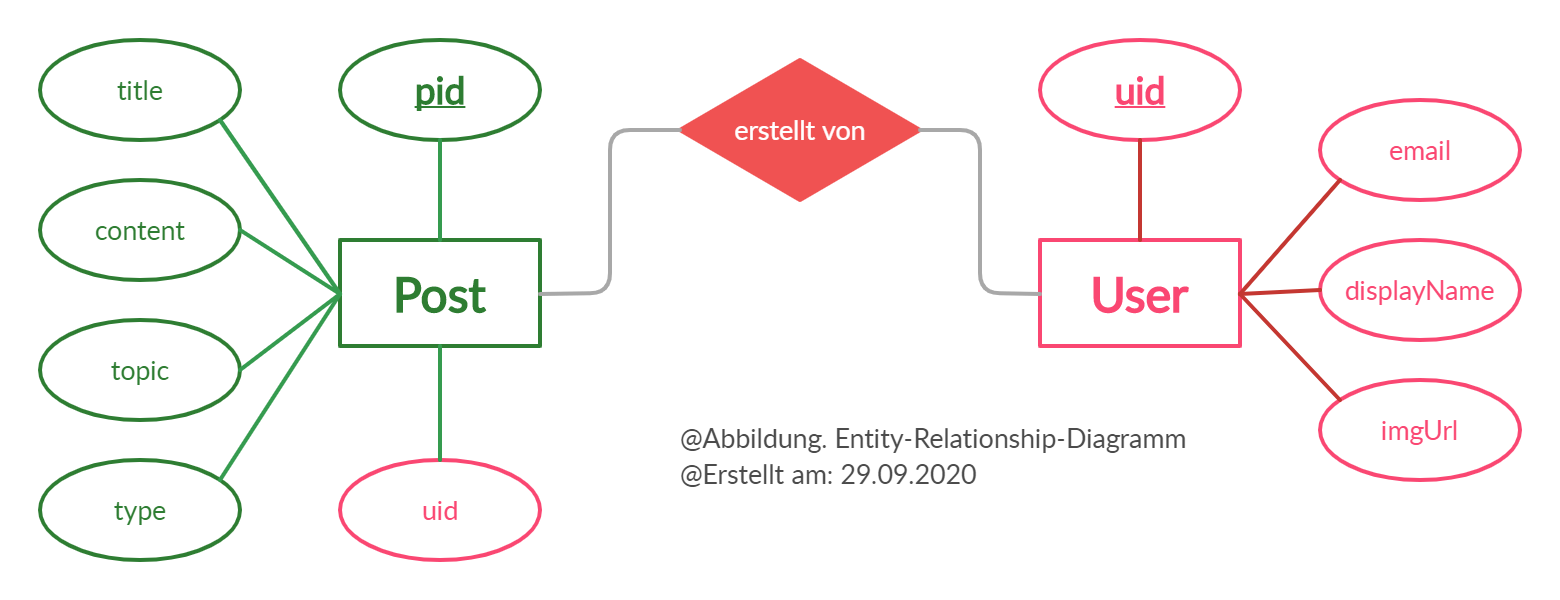
\includegraphics[width=400pt]{abbildungen/Abbildung_ERM.png}
\caption[ERM]{Entity Realationship Modell \\Quelle: eigene Darstellung}
\end{figure}

\FloatBarrier

\section{Fazit}
Insgesamt hat uns die LEA und das Arbeiten im Team sehr gut gefallen, allerdings empfanden wir das Prozedere als unorganisiert und nicht einheitlich von Seiten der Dozenten.\\

Die Verwendung einer neuen Programmiersprache und die Auseinandersetzung mit Webentwicklung war auf jeden Fall lehrreich und hat uns auf fachlicher Ebene weitergebracht. Dennoch halten wir es für unwahrscheinlich, dass wir uns in nächster Zeit nocheinmal freiwillig damit beschäftigen. \\

Für die nächste LEA haben wir uns vorgenommen unser Ziele geringer zu fassen und lieber wenige Kernfeatures voll auszubauen.

\subsection{Mögliche Erweiterung}

Insgesamt lässt sich das durch weitere Module oder Seiten ersetzen, wie andere Foren-Oberthemen, eine Stundenplanintegration über die ical- API oder 
ein Messengersystem für die User.
\newpage
\section{Quellen}

Wir haben folgende Seiten zur Hilfe genutzt:

\begin{itemize}
\item
Angular Dokumentation \\
https://angular.io/docs

 \item 
 Firebase Dokumentation \\
https://firebase.google.com/docs

\item
LazyLoading.gif \\ 
https://www.npmjs.com/package/angular-responsive-carousel

\item
Schema-generator  \\ 
http://colormind.io/bootstrap/

\item
Schriftart \\ 
https://fonts.google.com/specimen/Montserrat

\item
Stackoverflow \\
https://stackoverflow.com/

\item
Youtube \\
https://www.youtube.com

\end{itemize}


\end{document}
 
